\newif\ifstandalone
\standalonetrue % comment out for compilation with ktikz

\ifstandalone
\documentclass{standalone}
\fi

\usetikzlibrary{shapes.geometric, arrows, positioning, arrows.meta, calc}

\def\xconnection (#1,#2) {\draw[connection] (#1.north west) -- (#2.south east);  \draw[connection] (#1.north east) -- (#2.south west);}
\def\connection (#1,#2) {\draw[connection] (#1.north west) -- (#2.south west);  \draw[connection] (#1.north east) -- (#2.south east);}

\ifstandalone
\begin{document}
\fi

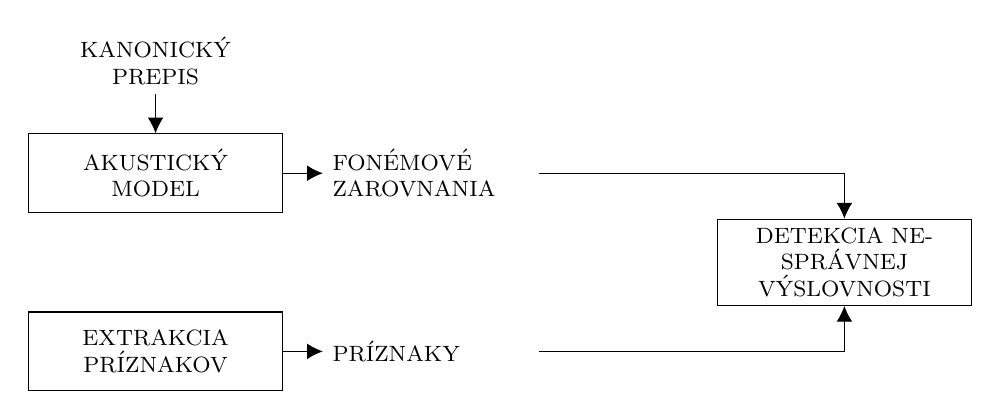
\begin{tikzpicture}[every node/.style = {font=\footnotesize}, node distance=2cm, >={Latex[width=2mm,length=2mm]}]
		\tikzstyle{punkt} = [rectangle, rounded corners, draw=black, very thick, text width=6.5em, minimum height=2em, text centered]
		\tikzstyle{pil} = [->,thick,shorten <= 2pt, shorten >= 2pt]
		\tikzstyle{block} = [rectangle, minimum width=3cm, minimum height=1cm, text centered, text width=3cm, draw=black]
		\tikzstyle{io} = [text width=2.5cm, align=flush left]
		% \tikzstyle{arrow} = [thick,->,>=stealth]
		\tikzstyle{arrow} = [->]

	    \node[block] (am) {AKUSTICKÝ MODEL};
        \node[io, text centered, above=0.5cm of am] (am-input) {KANONICKÝ PREPIS};
        \node[io, right=0.5cm of am] (am-output) {FONÉMOVÉ ZAROVNANIA};
        \node[below=0.5cm of am] (dummy) {};
        \node[block, below=0.5cm of dummy] (fe) {EXTRAKCIA PRÍZNAKOV};
        \node[io, right=0.5cm of fe] (fe-output) {PRÍZNAKY};
        \node[block, right=7cm of dummy] (md) {DETEKCIA NESPRÁVNEJ VÝSLOVNOSTI};
        \draw[arrow] (am) -- (am-output);
        \draw[arrow] (am-input) -- (am);
        \draw[arrow] (am-output) -| (md);
        \draw[arrow] (fe) -- (fe-output);
        \draw[arrow] (fe-output) -| (md);
\end{tikzpicture}

\ifstandalone
\end{document}
\fi